%---Escopo
%Apresentação da estrutura analítica do projeto (EAP)
%	ID
%	Nome
%	Entregas de GP
%	Sem filhos únicos
%	Tarefas x Pacotes
%---

%\begin{landscape}

\chapter{Estrutura Analítica do Projeto}\label{ch:wbs}

%\includepdf[pages=1,scale=.9,pagecommand={\chapter{Estrutura Analítica do Projeto}\label{ch:wbs}\todo[color=orange]{Criar diagrama para EAP para substituir relatório exportado do MS Project}},offset=0 -3cm,linktodoc=true]{include/eap.pdf}
%\includepdf[pages=2-,scale=.9,pagecommand={}]{include/eap.pdf}
\todo[inline,color=red]{Revisar EAP.}

\begin{figure}[h]
\centering
\begin{tikzpicture}[node distance = 0.3cm and 0.1cm, auto, scale=0.6, every node/.style={scale=0.6}]
	% Project management
	\node (project-management) [wbsblock] {Gerenciamento do projeto};
	\node (initiation) [wbsblock, below right= of project-management, xshift=-6em] {Iniciação};
	\node (planning) [wbsblock, below = of initiation] {Planejamento};
	\node (scope-approval) [wbsblock, below = of planning] {Aprovação do escopo};
	\node (project-monitoring) [wbsblock, below = of scope-approval] {Monitoramento do projeto};
	% Infraestrutura
	\node (infrastructure) [wbsblock, right = of project-management, xshift=1.5em] {Infraestrutura};
	\node (dev-env) [wbsblock, below right = of infrastructure, xshift=-6em] {Ambiente de desenvolvimento};
	\node (test-env) [wbsblock, below = of dev-env] {Ambiente de testes};
	\node (prod-env) [wbsblock, below = of test-env] {Ambiente de produção};
	% Banco de dados
	\node (database) [wbsblock, right = of infrastructure, xshift=1.5em] {Banco de dados};
	% Aplicativo do motorista
	\node (drivers-app) [wbsblock, right = of database, xshift=1.5em] {Aplicativo do motorista};
	\node (authentication) [wbsblock, below right = of drivers-app, xshift=-6em] {Autenticação};
	\node (spot-reservation) [wbsblock, below = of authentication] {Reserva de vagas};
	\node (parking-list) [wbsblock, below = of spot-reservation] {Lista de estacionamentos};
	\node (payment-process) [wbsblock, below = of parking-list] {Processamento de pagamento};
	\node (user-management) [wbsblock, below = of payment-process] {Gerência de usuário};
	% Aplicativo do estacionamento
	\node (parking-app) [wbsblock, right = of drivers-app, xshift=1.5em] {Aplicativo do estacionamento};
	\node (user-auth-management) [wbsblock, below right = of parking-app, xshift=-6em] {Autenticação e gerência de usuários};
	\node (client-management) [wbsblock, below = of user-auth-management] {Gerenciamento dos clientes};
	\node (system-register) [wbsblock, below = of client-management] {Solicitação de cadastro no sistema};
	\node (parking-management) [wbsblock, below = of system-register] {Gerenciamento do estacionamento};
	\node (garage-register) [wbsblock, below right = of parking-management, xshift=-6em] {Cadastro e gerência de garagens};
	\node (spot-state) [wbsblock, below = of garage-register] {Situação das vagas};
	\node (automation-integration) [wbsblock, below = of spot-state] {Integração com sistema de automação};
	\node (parking-configuration) [wbsblock, below = of automation-integration] {Configurações do estacionamento};
	\node (reports) [wbsblock, below left = of parking-configuration, xshift=6em] {Relatórios};
	\node (DETRAN-integration) [wbsblock, below = of reports] {Integração com DETRAN};
	% Auditoria
	\node (auditing) [wbsblock, right = of parking-app, xshift=1.5em] {Auditoria};
	\node (unit-test) [wbsblock, below right = of auditing, xshift=-6em] {Testes unitários};
	\node (integration-test) [wbsblock, below = of unit-test] {Testes de integração};
	% Encerramento
	\node (closure) [wbsblock, right = of auditing, xshift=1.5em] {Encerramento};
	% WBS root
	\node (free-spot) [wbsblock, above = of drivers-app, yshift=4em] {Vaga livre};

	\path [simpleline] (free-spot.south) |- ++(0,-1cm) -| (project-management);
	\path [simpleline] (free-spot.south) |- ++(0,-1cm) -| (infrastructure);
	\path [simpleline] (free-spot.south) |- ++(0,-1cm) -| (database);
	\path [simpleline] (free-spot.south) |- ++(0,-1cm) -| (drivers-app);
	\path [simpleline] (free-spot.south) |- ++(0,-1cm) -| (parking-app);
	\path [simpleline] (free-spot.south) |- ++(0,-1cm) -| (auditing);
	\path [simpleline] (free-spot.south) |- ++(0,-1cm) -| (closure);

	\path [simpleline] (project-management.215) |- (planning);
	\path [simpleline] (project-management.215) |- (scope-approval);
	\path [simpleline] (project-management.215) |- (project-monitoring);

	\path [simpleline] (infrastructure.215) |- (dev-env);
	\path [simpleline] (infrastructure.215) |- (test-env);
	\path [simpleline] (infrastructure.215) |- (prod-env);

	\path [simpleline] (drivers-app.215) |- (authentication);
	\path [simpleline] (drivers-app.215) |- (spot-reservation);
	\path [simpleline] (drivers-app.215) |- (parking-list);
	\path [simpleline] (drivers-app.215) |- (payment-process);
	\path [simpleline] (drivers-app.215) |- (user-management);

	\path [simpleline] (parking-app.215) |- (user-auth-management);
	\path [simpleline] (parking-app.215) |- (client-management);
	\path [simpleline] (parking-app.215) |- (system-register);
	\path [simpleline] (parking-app.215) |- (parking-management);
	\path [simpleline] (parking-app.215) |- (reports);
	\path [simpleline] (parking-app.215) |- (DETRAN-integration);
	\path [simpleline] (parking-management.215) |- (garage-register);
	\path [simpleline] (parking-management.215) |- (spot-state);
	\path [simpleline] (parking-management.215) |- (automation-integration);
	\path [simpleline] (parking-management.215) |- (parking-configuration);

	\path [simpleline] (auditing.215) |- (unit-test);
	\path [simpleline] (auditing.215) |- (integration-test);

\end{tikzpicture}
\caption{Estrutura analítica do projeto.}
\label{fig:wbs}
\end{figure}

%\end{landscape}